% Tema4.tex

\chapter{Variedades topológicas. Superficies}

\section{La topología cociente}

\defn{Topología final o imagen}{
    Sea \((X, \T)\) un espacio topológico, \(Y\) un conjunto y \(p: X \to Y\) una aplicación. Definimos en \(Y\) la topología final o imagen de \(p\) como:
    \[
    \T(p) := \{O \subset Y \mid p^{-1}(O) \in \T\}.
    \]
}
\clmp{}{
    $\T(p)$ es una topología sobre $Y$
}{
    \begin{enumerate}
    \item[(T1)] $p^{-1}(\emptyset)=\emptyset\in\T\implies\emptyset\in\T(p)$. $p^{-1}(Y)=X\in\T\implies Y\in\T(p)$.
    \item[(T2)] Si $U_i\in\T(p)\ \forall i\in I$ entonces $p^{-1}(U_i)\in\T\ \forall i\in I$, por tanto $p^{-1}(\bigcup_{i\in I}U_i)=\bigcup_{i\in I}p^{-1}(U_i)\in\T$ lo que significa que $\bigcup_{i\in I}U_i\in\T(p)$.
    \item[(T3)] Si $U_i\in\T(p)\ \forall i\in\{1,\dots,n\}$ entonces $p^{-1}(U_i)\in\T\ \forall i\in\{1,\dots,n\}$, por tanto $p^{-1}(\bigcap_{i=1}^{n}U_i)=\bigcap_{i=1}^{n}p^{-1}(U_i)\in\T$ lo que significa que $\bigcap_{i=1}^{n}U_i\in\T(p)$.
    \end{enumerate}
}


\propp{Propiedades de la topología final}{\label{prop:112}
    \begin{enumerate}
    \item \(\T(p)\) hace a \(p\) continua y es la topología más fina que lo hace.
    \item Sea \(g : (Y, \T(p)) \to (Z, \T'')\) una aplicación. \(g\) es continua si y solo si \(g \circ p\) es continua.  
    \item Los cerrados de \(\T(p)\) son \(\{C \subset Y \mid p^{-1}(C) \text{ es cerrado en } \T\}\).
    \end{enumerate}
}{
    \begin{enumerate}
        \item Que $\T(p)$ hace continua a $p$ es inmediato por la propia definición de $\T(p)$. Además, si $\T'$ es otra topología cualquiera que hace a $p$ continua entonces $\forall U\in\T', p^{-1}(U)\in\T\implies U\in\T(p)$, por lo que $\T'\subset\T(p)$, luego la topología final es la más fina.
        \item Claramente si $g$ es continua entonces $g\circ p$ es continua, puesto que es composición de dos aplicaciones continuas (recordemos que $p$ es continua como aplicación en $(Y,\T(p))$). Si por el contrario $g\circ p$ es continua, entonces dado $U\in\T''$ arbitrario, la preimagen $(g\circ p)^{-1}(U)=p^{-1}(g^{-1}(U))\in\T$ es abierta por ser $g\circ p$ continua, pero entonces por la definición de $\T(p)$ debe cumplirse $g^{-1}(U)\in\T(p)$, por tanto $g$ es continua.
        \item $C$ es cerrado en $\T(p) \iff Y\setminus C\in\T(p)\iff p^{-1}(Y\setminus C)\in\T \iff X\setminus p^{-1}(C)\in\T\iff p^{-1}(C)$ es cerrado en $\T$. El tercer $\iff$ se cumple puesto que $p^{-1}(Y)=X$.
    \end{enumerate}
}

\defn{Identificación}{
    Sean \((X, \T)\), \((Y, \T')\) espacios topológicos, y \(p: X \to Y\) una aplicación. Decimos que \(p : (X, \T) \to (Y, \T')\) es una identificación si \(p\) es sobreyectiva y \(\T' = \T(p)\).
}

\rmkb{Si $f:X\to Y$ es una aplicación sobreyectiva entonces $f(f^{-1}(U))=U$ para cualquier $U\subset X$.}

\propp{Propiedades de las identificaciones}{\label{prop:114}
    \begin{enumerate}
    \item \(Id : (X, \T) \to (X, \T')\) es una identificación si y solo si \(\T = \T'\).  
    \item Si \(p : (X, \T) \to (Y, \T')\) es una identificación y \(f : (Y, \T') \to (Z, \T'')\) es una aplicación, entonces \(f\) es continua si y solo si \(f \circ p\) es continua.
    \item Si \(f : (X, \T) \to (Y, \T')\) es continua, abierta (o cerrada) y sobreyectiva, entonces \(f\) es una identificación.
    \end{enumerate}
}{
    \begin{enumerate}
        \item Claramente $Id$ es sobreyectiva (de hecho es biyectiva con inversa $(Id)^{-1}=Id$), por lo que será identificación si y solo si $\T'=\T(Id)$. Ahora bien, $\T(Id)=\{O \subset Y \mid (Id)^{-1}(O) \in \T\}=\{O \subset Y \mid O \in \T\}=\T$, por tanto $Id$ es identificación si y solo si $\T'=\T$.
        \item Si $f$ es continua entonces $f\circ p$ es continua por ser composición de aplicaciones continuas. Si por el contrario $f\circ p$ es continua, entonces dado $U\in\T''$ arbitrario, la preimagen $(f\circ p)^{-1}(U)=p^{-1}(f^{-1}(U))\in\T$ es abierta por ser $f\circ p$ continua, pero entonces, como $\T'=\T(p)$ al ser $p$ identificación, debe cumplirse $f^{-1}(U)\in\T'$, por tanto $f$ es continua.
        \item Como $f$ es sobreyectiva solo necesitamos ver que si es continua y abierta (cerrada) entonces $\T'=\T(f)$. Supongamos que $f$ es continua, en tal caso tenemos garantizado que $\T'\subset\T(f)$.
        
        Si además es abierta entonces dado $U\in\T(f)$ arbitrario, $f^{-1}(U)\in\T$ por la definición de $\T(f)$, pero entonces $f(f^{-1}(U))\in\T'$ al ser $f$ abierta, y como es sobreyectiva $f(f^{-1}(U))=U\in\T'$, por lo que $\T(f)\subset\T'\subset\T(f)\implies \T(f)=\T'$, luego $f$ es una identificación.
        
        Si $f$ es cerrada razonamos de manera similar pero con cerrados: dado $U\in\T(f)$, $C=Y\setminus U$ es cerrado en $\T(f)$, por lo que $f^{-1}(C)$ es cerrado en $\T$\footnote{Por la tercera parte de la Proposición \hyperref[prop:112]{1.1.2}}, por tanto $f(f^{-1}(C))=C$ es cerrado en $\T'$ al ser $f$ cerrada, pero entonces $U=Y\setminus C\in\T'$, por tanto $\T(f)\subset\T'\subset\T(f)\implies \T(f)=\T'$, luego $f$ es una identificación.
    \end{enumerate}
}

\defn{Topología cociente}{
    Sea \((X, \T)\) un espacio topológico, \(\sim\) una relación de equivalencia en \(X\), y \(p: X \to \faktor{X}{\sim} = \tilde{X}\) la proyección al cociente. La topología cociente sobre \(\tilde{X}\) es la topología final o imagen de $p$:
    \[
    \faktor{\T}{\sim} = \tilde{\T} := \T(p) = \{ V \subset \tilde{X} \mid p^{-1}(V) \in \T \}.
    \]
    El espacio \((\tilde{X}, \tilde{\T})=(\faktor{X}{\sim},\faktor{\T}{\sim})\) se llama espacio cociente.
}

% \clmp{}{
%     $\tilde{\T}$ es una topología sobre $\tilde{X}$
% }{
%     Trivial.
% }

\rmkb{
    \begin{enumerate}
        \item  Toda relación de equivalencia \(\sim\) sobre \(X\) determina un espacio cociente dado por \(\tilde{X} = X / \sim\). Recíprocamente, todo espacio final asociado a una aplicación $p$ es el espacio cociente correspondiente a la relación de equivalencia $\sim_p$ dada por
        
        $x\sim_py\iff p(x)=p(y)$.
        \item Al definir un cociente estamos identificando los puntos que están en una misma clase de equivalencia.
        \item  \(\tilde{\T}\) es la topología más fina sobre \(\tilde{X}\) que hace continua a \(p\).
    \end{enumerate}
}

\propp{Propiedades del espacio cociente}{\label{prop:116}
    \begin{enumerate}
    \item \(V\) es un abierto de \(\tilde{X}\) si y solo si \(\bigcup_{[x] \in V}[x]\) es abierto en \(X\).  
    \item Si \(X\) es compacto, entonces \(\tilde{X}\) es compacto.  
    \item Si \(X\) es conexo (conexo por caminos), entonces \(\tilde{X}\) es conexo (conexo por caminos).
    \item $p:(X,\T)\to(\tilde{X},\tilde{\T})$ es una identificación.
    \item \(g : (\tilde{X}, \tilde{\T}) \to (Y, \T')\) es continua si y solo si \(g \circ p : (X, \T) \to (Y, \T')\) es continua.
    \end{enumerate}
}{
    \begin{enumerate}
        \item $V\in\tilde{\T}\iff p^{-1}(V)\in\T$ por definición de la topología cociente, veamos que $p^{-1}(V)=\bigcup_{[x] \in V}[x]$. Si $y \in p^{-1}(V) \implies p(y)=[y] \in V$, por tanto $[y]\subset\bigcup_{[x] \in V}[x]$, luego $y\in[y]\subset\bigcup_{[x] \in V}[x]$, por lo que $p^{-1}(V)\subset\bigcup_{[x] \in V}[x]$.
        
        Por otro lado si $x\in\bigcup_{[x] \in V}[x]$ entonces $[x]\in V$, por tanto $p(x)=[x] \in V \implies x \in p^{-1}(V)$, lo que prueba finalmente que $p^{-1}(V)=\bigcup_{[x] \in V}[x]$.
        \item Sabemos que la aplicación $p$ es continua y la compacidad se preserva por aplicaciones continuas. Como además $p$ es sobreyectiva entonces $p(X)=\tilde{X}$, por tanto si $X$ es compacto entonces $p(X)=\tilde{X}$ también lo es.
        \item Sabemos que la aplicación $p$ es continua y tanto la conexión como la arcoconexión se preservan por aplicaciones continuas. Como además $p$ es sobreyectiva entonces $p(X)=\tilde{X}$, por tanto si $X$ es conexo (conexo por caminos) entonces $p(X)=\tilde{X}$ también lo es.
        \item Es inmediato que $\tilde{\T}=\T(p)$, por otro lado dado $y\in\tilde{X}\implies y=[x]$ para cierto $x\in X$, por tanto $p(x)=y$, luego $p$ es sobreyectiva.
        \item Por el apartado 4, $p$ es una identificación, por tanto basta aplicar la parte 2 de la Proposición \hyperref[prop:114]{1.1.4}
    \end{enumerate}
}

Recordemos ahora que dada una aplicación $f:X\to Y$ cualquiera, podemos definir una relación de equivalencia sobre $X$ a partir de ella. Denotaremos por $R_f$ a la relación de equivalencia en $X$ dada por:
\[
x R_fx'\iff f(x)=f(x')
\]

\exer{
Demostrar que $R_f$ es una relación de equivalencia.
}

\thmr{Proposición 4.1}{diagrama}{
    Dados \((X, \T)\) y \((Y, \T')\) espacios topológicos, $f:(X, \T)\to(Y,\T')$ y \((\tilde{X}, \tilde{\T})\) el espacio cociente dado por \(R_f\), existe una aplicación \(\tilde{f} : (\tilde{X}, \tilde{\T}) \to (Y, \T')\) que hace que el siguiente diagrama sea conmutativo\footnote{Que el diagrama sea conmutativo quiere decir que ``da igual qué camino de flechitas sigamos'', es decir, $\tilde{f}\circ p=f$.}
    \begin{center}
        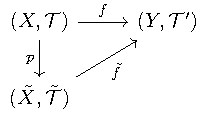
\includegraphics[]{otros/diagrama.pdf}
    \end{center}
    Además, \(f : (X, \T) \to (Y, \T)\) es una identificación si y solo si \(\tilde{f} : (\tilde{X}, \tilde{\T}) \to (Y, \T')\) es un homeomorfismo.
}
\pf{
    Si pretendemos que el diagrama sea conmutativo debe cumplirse
    \[
    \tilde{f}(p(x))=f(x)
    \]
    Es decir,
    \[
        \tilde{f}([x])=f(x)
    \]
    Por tanto definimos $\tilde{f}$ de la siguiente manera:
    \[
    \tilde{f}:(\tilde{X}, \tilde{\T}) \to (Y, \T'),\quad \tilde{f}([x])=f(x).
    \]
    Ahora solo necesitamos ver que la aplicación está bien definida\footnote{Una aplicación que tiene como dominio un cociente está bien definida si la imagen de una clase de equivalencia no depende del representante escogido para la clase.}. En efecto si $x,y\in X$ son dos representantes de la misma clase de equivalencia $[x]$ entonces $xR_fy$, por tanto se cumple $f(x)=f(y)$, luego
    \[
    \tilde{f}([x])=f(x)=f(y)=\tilde{f}([y])
    \]
    por lo que la aplicación está bien definida.

    Para la segunda parte, si suponemos que $\tilde{f}$ es un homeomorfismo entonces $f=\tilde{f}\circ p$ es continua por ser composición de funciones continuas, y es sobreyectiva por serlo $\tilde{f}$ y $p$. Además, si $U\in\T(f)$ entonces $f^{-1}(U)=p^{-1}(\tilde{f}^{-1}(U))\in\T$, por tanto $\tilde{f}^{-1}(U)\in\tilde{\T}$, y al ser $\tilde{f}$ abierta y biyectiva  $U=\tilde{f}(\tilde{f}^{-1}(U))\in\T'$, lo que prueba que $\T(f)=\T'$ y por tanto $f$ es una identificación.

    Si por el contrario suponemos que $f$ es una identificación entonces $f$ es sobreyectiva y $\T'=\T(f)$, por tanto $f$ es continua y al ser $p$ identificación también lo es $\tilde{f}$ (apartado 2 de la Proposición \hyperref[prop:114]{1.1.4}). Que $\tilde{f}$ es inyectiva es inmediato por  la propia definición de $\tilde{f}$. Para ver que es sobreyectiva, dado $y\in Y$ por ser $f$ sobreyectiva existe $x\in X\mid f(x)=y$, por tanto $\exists z=[x]\in\tilde{X}$ tal que $\tilde{f}([x])=f(x)=y$. Veamos que $\tilde{f}$ es abierta: dado $U\in\tilde{\T}$ entonces $f^{-1}(\tilde{f}(U))=p^{-1}(\tilde{f}^{-1}(\tilde{f}(U)))=p^{-1}(U)\in\T$ por ser $p$ continua, por lo tanto $\tilde{f}(U)\in\T(f)=\T'$, luego $\tilde{f}$ es un homeomorfismo.
}

\clearpage

\section{Ejemplos de espacios cocientes}\label{sec:ejemplos-cocientes}

Veamos ahora algunos ejemplos de espacios cociente y la posibilidad de establecer homeomorfismos entre estos espacios cociente y otros espacios topológicos de interés. En estos primeros ejemplos haremos uso del Teorema \ref{thm:diagrama} para encontrar tales homeomorfismos.

\ex{
    Para el intervalo \(I = [0, 1]\), consideramos la partición:
    \[
    \tilde{I} = \{ \{0, 1\} \} \cup \{ \{x\} : x \in (0, 1) \}.
    \]
    El espacio cociente \((\tilde{I}, \tilde{\T})\) es homeomorfo a la circunferencia unidad \( \sphere^1 \).
}
\pf{
    Probemos que la relación $\sim$ dada por la partición $\tilde{I}$ coincide con la relación dada por la aplicación $f:I\to\sphere^1, f(t)=(\cos(2\pi t),\sin(2\pi t))$. Para ello, dados $x,y\in I$
    \[
    x R_f y \iff f(x)=f(y) \iff
    \begin{cases}
    \cos(2\pi x)=\cos(2\pi y)\\
    \sin(2\pi x)=\sin(2\pi y)
    \end{cases}
    \]
    Para que se den estas igualdades entre cosenos y senos hay varias opciones: si $x,y\in(0,1)$ entonces debe cumplirse $x=y$; si $x,y\in\{0,1\}$ entonces o bien $x=y$, o bien $x=0,y=1$, o bien $x=1,y=0$. En resumen:
    \[
    x R_f y \iff x=y \text{  o  } x=1,y=0 \text{  o  } x=0,y=1\iff x\sim y 
    \]
    Por tanto ambas son la misma relación. Ahora veamos que $f$ es una identificación, y por tanto $\exists \tilde{f}$ homeomorfismo entre $\tilde{I}$ y $\sphere^1$.

    En primer lugar, $f$ es continua por ser restricción de una aplicación continua (basta considerarla como aplicación de $I$ a $\R^2$), además es cerrada puesto que $I$ es compacto y $\sphere^2$ es Hausdorff (Ver Ejercicio \hyperref[exer:12]{1.2}). Por último dado $(x,y)\in\sphere^1$, denotemos por $\alpha=\text{ang}((x,y))$ al ángulo en radianes que forma el punto $(x,y)$ con la horizontal, con $\alpha\in[0,2\pi)$. Es sencillo comprobar que $f(\frac{\alpha}{2\pi})=(x,y)$, por tanto $f$ es sobreyectiva, lo que según la Proposición \hyperref[prop:114]{1.1.4} apartado 3 garantiza que $f$ es una identificación, y por tanto $\exists \tilde{f}$ homeomorfismo entre $\tilde{I}$ y $\sphere^1$
}

\exer{Probar que si $X$ es compacto, $Y$ es Hausdorff y $f:(X,\T)\to(Y,\T')$ es continua entonces $f$ es cerrada.}\label{exer:12}


\ex{
    Sea \(X = [0, 1] \times [0, 1]\) con la relación de equivalencia:
    \[
    (x_1, y_1) \sim (x_2, y_2) \text{ si y solo si } x_1 - x_2 \in \mathbb{Z} \text{ e } y_1 = y_2.
    \]
    El espacio cociente es homeomorfo a un cilindro.
}

\pf{
    Consideremos el cilindro $C=\{(x,y,z)\in\R^3 \mid x^2+y^2=1, z\in[0,1]\}$, probaremos que la relación $\sim$ coincide con la relación dada por la aplicación $f:X\to C, f(t,s)=(\cos(2\pi t),\sin(2\pi t),s)$. Para ello, dados $(x_1,y_1),(x_2,y_2)\in X$
    \[
        (x_1,x_2) R_f (x_2,y_2) \iff
        \begin{cases}
        \cos(2\pi x_1)=\cos(2\pi x_2)\\
        \sin(2\pi x_1)=\sin(2\pi x_2)\\
        y_1=y_2
        \end{cases}
    \]
    Dejamos como un sencillo ejercicio comprobar que para que se den estas igualdades entre cosenos y senos debe darse $x_1-x_2\in\mathbb{Z}$. En resumen:
    \[
        (x_1,x_2) R_f (x_2,y_2) \iff (x_1,y_1)\sim(x_2,y_2)
    \]
    Por tanto ambas son la misma relación. Ahora veamos que $f$ es una identificación, y por tanto $\exists \tilde{f}$ homeomorfismo entre $\tilde{X}$ y $C$.

    En primer lugar, $f$ es continua y cerrada por un argumento similar al del ejemplo anterior. Para ver que es sobreyectiva basta tomar $p=(x,y,z)\in C$, y denotemos por $\alpha=\text{ang}((x,y))$ al ángulo en radianes que forma el punto $(x,y)$ con la horizontal si consideramos a $(x,y)$ como punto de $\sphere^1$, con $\alpha\in[0,2\pi)$. Entonces $f(\frac{\alpha}{2\pi},z)=(x,y,z)=p$, por lo que $f$ es sobreyectiva y por tanto identificación.
}

\clearpage
\ex{
    Sea \(X = [0, 1] \times [0, 1]\) con la relación de equivalencia:
    \[
    (x_1, y_1) \sim (x_2, y_2) \text{ si y solo si } (x_1, y_1) = (x_2, y_2) \text{ o } [x_1 - x_2 = \pm 1 \text{ e } y_1 = 1 - y_2].
    \]
    El espacio cociente es homeomorfo a una banda de Möbius.
}

\pf{
    Llamamemos $M$ a la banda de Möbius. $M$ será la imagen de la función 
    \begin{gather*}
        F:[0,2\pi]\times[-1,1]\to\R^3 \\
        F(u,v)=((2-v\sin(\frac{u}{2}))\sin(u),(2-v\sin(\frac{u}{2}))\cos(u),v\cos(\frac{u}{2}))
    \end{gather*}
    es decir, $M=F([0,2\pi]\times[-1,1])$.

    Probaremos ahora que la función $f:I\times I\to M$ dada por $f(t,s)=F(2\pi t,2s-1)$ define la misma relación que $\sim$ y además es una identificación. La aplicación f es claramente continua, cerrada por ir de un compacto a un $T_2$ y sobreyectiva por definición (ya que $M=F([0,2\pi]\times[-1,1])=f(I\times I))$.
    
    En cuanto a la relación, dados $(x,y),(a,b)\in I\times I$
    \begin{gather*}
        (x_1,y_1)R_f(x_2,y_2) \iff f(x_1,y_1)=f(x_2,y_2) \iff\\
        \iff \begin{cases}
            (2-(2y_1-1)\sin(\pi x_1))\sin(2\pi x_1) =  (2-(2y_2-1)\sin(\pi x_2))\sin(2\pi x_2)\\
            (2-(2y_1-1)\sin(\pi x_1))\cos(2\pi x_1) = (2-(2y_2-1)\sin(\pi x_2))\cos(2\pi x_2) \\
            (2y_1-1)\cos(\pi x_1) = (2y_2-1)\cos(\pi x_2)
        \end{cases}
    \end{gather*}
    claramente si $(x_1, y_1) = (x_2, y_2) \text{ o } [x_1 - x_2 = \pm 1 \text{ e } y_1 = 1 - y_2]$ entonces se dan las igualdades y $(x_1,y_1)R_f(x_2,y_2)$. Por el contrario, si $(x_1,y_1)R_f(x_2,y_2)$ dejamos la comprobación de que debe cumplirse $(x_1, y_1) = (x_2, y_2) \text{ o } [x_1 - x_2 = \pm 1 \text{ e } y_1 = 1 - y_2]$ como ejercicio (o castigo) al lector.
}

\clearpage
\ex{
    Sea \(X = [0, 1] \times [0, 1]\) con la relación de equivalencia:
    \[
    (x_1, y_1) \sim (x_2, y_2) \text{ si y solo si } x_1 - x_2 \in \mathbb{Z} \text{ e } y_1 - y_2 \in \mathbb{Z}.
    \]  
    El espacio cociente es homeomorfo a un toro.
}

\pf{
    En primer lugar notemos que la relación de equivalencia consiste en identificar los lados del cuadrado $[0, 1] \times [0, 1]$ según la siguiente figura
    \begin{center}
        \includegraphics[width=0.2\textwidth]{img/cociente-toro.png}
    \end{center}
    En cuanto al toro $\mathbb{T}^2$, lo consideraremos como el subconjunto de $\R^3$ de la siguiente forma
    \[
    \mathbb{T}^2=\{(x,y,z)\in\R^3 \mid (\sqrt{x^2+y^2}-2)^2+z^2=1\}
    \]
    Si definimos la función
    \begin{gather*}
        F:[0,2\pi]\times[0,2\pi]\to\mathbb{T}^2 \\
        F(u,v)=(\cos u(\cos v+2),\sin u(\cos v+2),\sin v)
    \end{gather*}
    basta comprobar que
    \[
    f:[0,1]\times[0,1]\to \mathbb{T}^2,\quad f(t,s)=F(2\pi t,2\pi s)
    \]
    induce la misma relación de equivalencia que $\sim$, y además es continua, sobreyectiva y cerrada (por ir de un compacto a un Hausdorff). Todas estas comprobaciones, muy similares a las de los anteriores ejemplos, quedan como un sencillo ejercicio para el lector.
}

\clearpage

\ex{
    Sea \(X = [0, 1] \times [0, 1]\) con la relación de equivalencia:
    \[
    (x_1, y_1) \sim (x_2, y_2) \text{ si y solo si } [x_1 = x_2 \text{ e } y_1 - y_2 \in \mathbb{Z}] \text{ o } [x_1 - x_2 = \pm 1 \text{ e } y_1 = 1 - y_2].
    \]
    El espacio cociente es homeomorfo a una botella de Klein.
}

\pf{
    Definiremos la botella de Klein $K$ como el subconjunto de $\R^4$ dado por la imagen de la siguiente función:
    \begin{gather*}
        f:[0,1]\times[0,1]\to K\subset \R^4 \\
        f(t,s)=
        ((2+\cos(2\pi t))\cos(2\pi s),\\
        (2+\cos(2\pi t))\sin(2\pi s),\\
        \sin(2\pi t)\cos(\pi s),\\
        \sin(2\pi t)\sin(\pi s))
    \end{gather*}
    Claramente $f$ es continua, sobreyectiva (por la propia definición de $K$) y cerrada (por ir de un compacto a un $T2$). Además, se puede comprobar que determina la misma relación de equivalencia que $\sim$, por lo que en virtud de la Proposición 4.1 existe un homeomorfismo entre $\tilde{X}$ y la botella de Klein.
}

\clearpage

\ex{
    Sea \(X = \mathbb{S}^1 \times [0, 1]\) con la relación de equivalencia:
    \[
    (x_1, y_1) \sim (x_2, y_2) \text{ si y solo si } y_1 = y_2 = 0 \text{ o } (x_1, y_1) = (x_2, y_2).
    \]
    El espacio cociente es homeomorfo a un cono.
}

\pf{
    Definamos el cono
    \[
    C=\{(x,y,z)\in\R^3\mid x^2+y^2=z^2,z\in[0,1]\}
    \]
    y tomemos la función
    \begin{gather*}
        f:\sphere^1\times[0,1]\to C\\
        f(\theta,t)=(t\theta_x,t\theta_y,t),\quad \theta=(\theta_x,\theta_y)\in\sphere^1\subset\R^2
    \end{gather*}
    es inmediato ver que la función es continua, sobreyectiva y cerrada por argumentos como los del resto de ejemplos. Por otro lado
    \[
    (\theta,t)R_f(\theta',t')\iff t=t', t\theta=t'\theta' \iff t=t'=0\quad \text{ó} \quad (\theta,t)=(\theta',t')\iff (\theta,t)\sim(\theta',t')
    \]
    Por tanto existe un homeomorfismo entre $C$ y $\tilde{X}$.
}

\clearpage

\ex{
    Sea \(X = \mathbb{S}^2\) con la relación de equivalencia:
    \[
    p \sim q \iff p = \pm q.
    \]
    El espacio cociente $\tilde{\mathbb{S}}^2$ es homeomorfo al plano proyectivo \(\mathbb{RP}^2\).
}

\pf{
    En primer lugar, el plano proyectivo $\mathbb{RP}^2$ será el conjunto cociente obtenido al considerar la siguiente relación $\sim_p$ sobre $\R^3\setminus\{0\}$. 
    \[
    x \sim_p y\iff x=\lambda y, \lambda\neq 0.
    \]
    La idea va a ser construir una aplicación de $\R^3\setminus\{0\}$ a $\mathbb{S}^2$ de tal manera que la aplicación respeta la relación que existe sobre $\mathbb{S}^2$, es decir, $x\sim_p y\iff f(x)\sim f(y)$. Similarmente, veremos que existe una aplicación de $\mathbb{S}^2$ a $\R^3\setminus\{0\}$ que también respeta la relación de equivalencia del proyectivo. Esto garantiza que las aplicaciones ``pasan al cociente''. Finalmente veremos que estas aplicaciones en el cociente son homeomorfismos y que la una es la inversa de la otra. La idea se resume en el siguiente diagrama, donde $\pi_1,\pi_2$ son las proyecciones a los cocientes.
    \begin{center}
        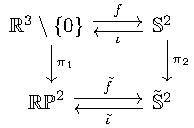
\includegraphics[width=0.25\textwidth]{otros/diagrama-proyectivo-esfera.pdf}
    \end{center}

    Definamos $f:\R^3\setminus\{0\}\to\sphere^2$ por $f(x)=\frac{x}{|x|}$, y $\iota:\sphere^2\to\R^3\setminus\{0\}$ por $\iota(x)=x$. Notemos que si $x,y\in\R^3\setminus\{0\}$ están relacionados entonces:
    \[
    x\sim_p y\iff x=\lambda y,\lambda\neq 0 
    \]
    y por tanto
    \[
    f(x)=\frac{x}{|x|}=\frac{\lambda y}{|\lambda||y|}=\pm\frac{y}{|y|}=\pm f(y) \iff f(x)\sim f(y).
    \]
    Además, si $f(x)\sim f(y)$ entonces 
    \[
    \frac{x}{|x|}=\pm\frac{y}{|y|}\implies x=\lambda y, \lambda \ne 0
    \]
    en esencia hemos visto que $x\sim_p y\iff f(x)\sim f(y)$, lo que garantiza que la aplicación $\tilde{f}([x]_p)=[f(x)]$\footnote{Usamos $[\cdot]_p$ para referirnos a las clases de equivalencia en el proyectivo y $[\cdot]$ para las clases de equivalencia en $\sphere^2$.} está bien definida puesto que
    \[
        \tilde{f}([x]_p)=\tilde{f}([y]_p)\iff [f(x)]=[f(y)]\iff f(x)\sim f(y) \iff x\sim_p y\iff [x]_p=[y]_p.
    \]
    La demostración de que $\iota$ también pasa al cociente como $\tilde{\iota}([x])=[\iota(x)]_p$ se deja como un sencillo ejercicio.
    
    Veamos ahora que $\tilde{f}$ y $\tilde{\iota}$ son inversas la una de la otra
    \[
    \tilde{f}(\tilde{\iota}([x]))=\tilde{f}([x]_p)=[f(x)]=\left[\frac{x}{|x|}\right]=[x]
    \]
    donde la última igualdad se sigue de que $x\in\sphere^2$ y por tanto $|x|=1$. Por otro lado
    \[
    \tilde{\iota}(\tilde{f}([x]_p))=\tilde{\iota}([f(x)])=\tilde{\iota}(\left[\frac{x}{|x|}\right])=\left[\frac{x}{|x|}\right]_p=[x]_p
    \]
    donde la última igualdad se sigue del hecho de que $\frac{x}{|x|}\sim_p x$.

    Veamos ahora que $\tilde{f}$ es continua. Para ello notemos que por la Proposición \hyperref[prop:116]{1.1.6}, $\tilde{f}$ es continua si y solo si $\tilde{f}\circ\pi_1=\pi_2\circ f$ lo es. Pero claramente $f$ es continua y también lo es la proyección $\pi_2$, por lo que $\tilde{f}$ es continua. De manera similar, $\iota$ es continua si y solo si lo es $\iota\circ\pi_2=\pi_1\circ\iota$, que es claramente continua por serlo $\pi_1, \iota$.

}

\clearpage

\ex{
    En el disco cerrado \(D(0, 1)\) de \(\mathbb{R}^2\), consideramos la relación de equivalencia:
    \[
    (x_1, y_1) \sim (x_2, y_2) \text{ si y solo si } (x_1,y_1),(x_2,y_2)\in\partial D(0,1), x_1 = \pm x_2 \text{ e } y_1 = y_2.
    \]
    El espacio cociente \(\faktor{D(0, 1)}{\sim}\) es homeomorfo a la esfera \(\mathbb{S}^2\).
}

\pf{
    Se deja como ejercicio.
}

\exer{
    Dado $(X,\T)$ un espacio topológico y $K\subset X$, definimos la relación
        \[
            x \sim y\iff
            \begin{cases}
                x,y \in K \\
                x=y
            \end{cases}
        \]
    y llamemos al espacio cociente $(\faktor{X}{K},\faktor{\T}{K}):=(\faktor{X}{\sim},\faktor{\T}{\sim})$.
        \begin{enumerate}
            \item[a)] Demostrar que $p|_{X\setminus K}:X\to p(X\setminus K)$ es una biyección.
            \item[b)] Demostrar que $p|_{X\setminus K}$ es un homeomorfismo si $K$ es abierto o cerrado.
        \end{enumerate}
}

\noindent\textbf{Solución:}

Para el apartado a) notemos que
\[
    \forall x \in X \setminus K,\quad p|_{X\setminus K}(x)=[x]
\]
pero por la manera en la que está definida la relación de equivalencia, es inmediato ver que $[x]=\{x\}$, ya que el único elemento relacionado con $x$ es el propio $x$ (recordemos que $x\notin K$). Por tanto $p|_{X\setminus K}$ es inyectiva ya que
\[
    p|_{X\setminus K}(x)=p|_{X\setminus K}(y)\implies [x]=[y]\implies \{x\}=\{y\}\implies x=y
\]
y además es sobreyectiva por estar definida en su imagen. Por tanto $p|_{X\setminus K}$ es una biyección.

Para el apartado b) notemos en primer lugar que $p$ es continua, por lo que $p|_{X\setminus K}$ también lo será por ser su restricción a $X\setminus K$.

Haremos el caso $K$ cerrado, cuando $K$ es abierto hay que razonar de manera idéntica pero con cerrados teniendo en cuenta la parte 3 de la Proposición \hyperref[prop:112]{1.1.2}.

Si  $K$ es cerrado entonces $X\setminus K$ es abierto, ahora si tomamos $U\in\T|_{X\setminus K}$ entonces $U=\tilde{U}\cap (X\setminus K), \tilde{U}\in\T$. Pero como $X\setminus K$ es abierto entonces de hecho $U\in\T$ y por tanto
\[
p^{-1}(p(U))=(p|_{X\setminus K})^{-1}(p|_{X\setminus K}(U))=U\in\T
\]
(recordemos que $p|_{X\setminus K}$ es una biyección y por tanto tiene inversa).
Finalmente por la definición de topología cociente debe de ser $p(U)\in\faktor{\T}{K}$, pero como además $p|_{X\setminus K}(U)=p(U)=p(U)\cap p(X\setminus K)$ deducimos que $p|_{X\setminus K}(U)\in\faktor{\T}{K}|_{p(X\setminus K)}$, lo que prueba que $p|_{X\setminus K}$ es abierta y por tanto un homeomorfismo.

\clearpage

\section{Espacios localmente euclídeos}

\defn{Espacio localmente euclídeo}{
    Un espacio topológico \((X, \T)\) se dice que es localmente euclídeo de dimensión \(n\) si todo punto \(p\) de \(X\) tiene un entorno \(U\) homeomorfo a una bola abierta \(B\) de \(\mathbb{R}^n\). Si \(\varphi: U \subset X \to B \subset \mathbb{R}^n\) es tal homeomorfismo, \((U, \varphi)\) se llama carta en \(X\) alrededor de \(p \in U\).
}

\rmkb{
    \begin{enumerate}
        \item Por ser \(X\) localmente euclídeo, este hereda las propiedades locales de \(\mathbb{R}^n\).
        \item Podemos sustituir la bola abierta en la definición anterior por un entorno abierto de \(\mathbb{R}^n\).
    \end{enumerate}
}

\defn{Bola euclídea}{
    Diremos que \(B' \subset X\) es una bola euclídea si $B'$ es homeomorfo a una bola abierta $B(0,r)$ de $\R^n$.
}

\defn{Bola regular euclídea}{
    Diremos que \(B \subset X\) es una bola regular euclídea si:
    \begin{itemize}
        \item Existe una bola euclídea \(B'\) tal que \(\overline{B} \subset B'\).
        \item Existe \(r > 0\) y una carta \(\varphi: B' \to B^n(0, 2r)\) tal que \(\varphi(\overline{B}) = \overline{B^n(0, r)}\).
    \end{itemize}
}

\section{Variedades topológicas}

\defn{Variedad topológica}{
    Una variedad topológica \(M\) es un espacio topológico \(T_2\) y \(2A\N\) que es localmente euclídeo de dimensión $n$. La dimensión de \(M\) es el número natural \(n\). También se denomina \(n\)-variedad (topológica).
}

\defn{Superficie topológica}{
    Una superficie topológica \(S\) es una variedad topológica de dimensión dos o 2-variedad.
}

\rmkb{
    En ocasiones podemos referirnos a las superficies topológicas como superficies, o en general a las $n$-variedades topológicas como $n$-variedades (o incluso variedades si se sobrentiende su dimensión). Cabe destacar que en otro contextos la palabra superficie puede referirse a un concepto distinto, como el de superficie parametrizada o el de variedad diferenciable de dimensión 2 (superficie regular).
}

\defn{Variedad con borde}{
    Si en la definición de variedad cambiamos el espacio modelo \(\mathbb{R}^n\) por el semiespacio superior \(\mathbb{H}^n = \{x \in \mathbb{R}^n : x_i \geq 0\}\), obtenemos el concepto de variedad con borde.
}

\ex{
    Sea $X=(\R\times\{0\})\cup(\R\times\{1\})$ y consideremos la relación $R$ dada por
    \[
    (x,0)R(x,1) \forall x\neq 0, (x,y)R(x,y) \forall (x,y)\in X.
    \]
    Entonces $\faktor{X}{R}$ es localmente euclídeo de dimensión 1 pero no es Hausdorff, por tanto no es una variedad. Para más información consultar \textit{Line with two origins} en Wikipedia.
}

\propp{Observaciones sobre variedades topológicas}{
    \begin{enumerate}
    \item Toda variedad topológica es localmente conexa por caminos (y localmente conexa).
    \item Las componentes conexas y las componentes conexas por caminos coinciden en una variedad.
    \item Una variedad es conexa si y solo si es conexa por caminos.
    \item Toda variedad es localmente compacta.
    \item Si una variedad no es compacta, siempre podremos compactificarla añadiendo un solo punto.
    \end{enumerate}
}{
  Sea $M$ una n-variedad. Notemos en primer lugar la siguiente afirmación que usaremos para probar el punto 4:
  \clmp{}{
     Dado $x\in M$, como $M$ es una variedad existe un entorno $U\in\E(x)$ homeomorfo a una bola $B(0,r)=\varphi(U)$ de $\R^n$ con $\varphi(x)=0$.
  }{
    Sabemos por ser $M$ variedad que existe un entorno $U'\in\E(x)$ y un homeomorfismo 
    
    \noindent$\psi:U'\to B$ con $B$ una bola en $\R^n$. Si $\psi(x)=0$ ya hemos acabado, si $\psi(x)\neq 0$ entonces podemos elegir una bola centrada en $\psi(x)$ de radio $r'$ lo suficientemente pequeño de manera que $B(\psi(x),r')\subset B\implies A=\psi^{-1}(B(\psi(x),r'))\subset\psi^{-1}(B)=U$, y $A\in\E(x)$. Finalmente la aplicación $\phi:B(\psi(x),r')\to B(0,r'), \phi(s)=s-\psi(x)$ es un homeomorfismo, por lo que $\varphi=\phi\circ\psi|_{A}:A\to B(0,r')$ es el homeomorfismo buscado.
  }

  De hecho dado cualquier $V\in\E(x)$ siempre podemos elegir el entorno homeomorfo a una bola de manera que $U\subset V$ puesto que si $U\not\subset V$, entonces basta tomar $B'(0,r')\subset B(0,r)$ lo suficientemente pequeña para que $U'=\varphi^{-1}(B'(0,r'))\subset U\cap V$ y claramente $U'$ también es homeomorfo a una bola de $\R^n$.
    \begin{enumerate}
      \item Sean $x\in M, V\in\E(x)$, como $M$ es una variedad existe un entorno $U\in\E(x),U\subset V$ homeomorfo a una bola de $\R^n$, y por tanto localmente conexo por caminos. Como $U$ es localmente conexo por caminos $\exists U'\subset U$ un entorno de $x$ conexo por caminos. Por último notemos que $U'\subset U\subset V\implies U'\subset V$, luego $U'$ es un entorno de $x$ conexo por caminos contenido en $V$, lo que prueba que $M$ es localmente conexa por caminos. Que es localmente conexa es inmediato puesto que localmente conexo por caminos implica localmente conexo. 
      \item Se sigue de las propiedades generales de un espacio localmente conexo por caminos.
      \item Se sigue de las propiedades generales de un espacio localmente conexo por caminos.
      \item Sea $x\in M$, como $M$ es una variedad existe un entorno $U\in\E(x)$ homeomorfo a una bola $B(0,r)$ mediante un homeomorfismo $\varphi : B(0,r)\rightarrow U $ con $\varphi(0) = x$. Puesto que $\overline{B(0,\frac{r}{2})}$ es compacto y $\varphi$ es continua, $\varphi(\overline{B(0,\frac{r}{2})})$ es un compacto. Además $\varphi(\overline{B(0,\frac{r}{2})})\subset\varphi(B(0,r))=U$ por lo que si tomamos $C=\varphi(\overline{B(0,\frac{r}{2})})$ como compacto y $U$ como entorno se verifica que $x\in C\subset U$, por lo que $M$ es localmente compacta en $x$, como el punto elegido era arbitrario $M$ es localmente compacta.
      \item Como cualquier variedad es $T_2$ y localmente compacta, verifica las hipótesis del Teorema de Alexandroff. Por tanto, en virtud de este resultado se puede compactificar por un punto.
    \end{enumerate}
}

\clearpage

\subsection{Ejemplos de superficies}

En todos los ejemplos siguientes consideramos subespacios de algún $\R^m$, por tanto todos los espacios son $T_2$ y $2A\N$ (recordemos que estas propiedades se heredan al considerar las topologías relativas). Solo necesitamos probar que cada uno de estos espacios son localmente euclídeos.

\ex{
  La esfera \(\mathbb{S}^2\) es una superficie topológica.
}

\pf{
    Sea $p=(x_0,y_0,z_0)\in\sphere^2$ y supongamos que $z_0>0$, en tal caso el entorno $U=\sphere^2\cap\{z>0\}$ es homeomorfo a la bola $B^2((0,0),1)$ mediante el homeomorfismo
    \[
    \varphi:B^2((0,0),1)\to U,\quad \varphi(x,y)=(x,y,\sqrt{x^2+y^2}).
    \]
    En efecto $\varphi$ es un homeomorfismo pues es abierta, continua y biyectiva, con inversa
    \[
    \varphi^{-1}(x,y,z)=(x,y).
    \]
    Para el resto de puntos sabemos que alguna de las tres componentes $x_0,y_0,z_0$ debe ser no nula, por lo que podemos hacer un procedimiento similar, tarea que encomendamos al lector.
}

\ex{
    El toro \(\mathbb{T}^2 = \mathbb{S}^1 \times \mathbb{S}^1\) es una superficie topológica.
}

\pf{
    Recomendamos al lector que vuelva a echar un vistazo al ejemplo referente al toro en la \hyperref[sec:ejemplos-cocientes]{Sección 1.2}, aunque en este caso identificaremos al toro con el producto cartesiano de dos circunferencias.
    
    Para ver que $\mathbb{T}^2$ es localmente euclídeo sea $p=(x_0,y_0)\in\mathbb{T}^2=\sphere^1\times\sphere^1$, de manera que
    \[
    p=((\cos\theta_0,\sin\theta_0),(\cos\phi_0,\sin\phi_0))
    \]
    para ciertos $\theta_0,\phi_0\in[0,2\pi)$. Consideremos la bola abierta $B=B((\theta_0,\phi_0),1)\subset\R^2$ y el homeomorfismo
    \[
    \varphi:B\to U\subset\sphere^1\times\sphere^1,\quad \varphi(\theta,\phi)=((\cos\theta,\sin\theta),(\cos\phi,\sin\phi)).
    \]
    En efecto es un homeomorfismo al considerarla sobre su imagen $U=\varphi(B)$ porque es continua y biyectiva con inversa continua. Que es sobreyectiva es inmediato, que es inyectiva también puesto que las funciones seno y coseno son $2\pi$-periódicas y el radio de la bola es menor que $2\pi$. Por tanto para cada punto $p$ existe la carta $(U,\varphi^{-1})$ en torno a ese punto, lo que prueba que $\mathbb{T}^2$ es localmente euclídeo.
}

\clearpage

\ex{
    El cilindro \(\mathbb{S}^1 \times \mathbb{R}\) es una superficie topológica.
}

\pf{
    Sea $p=((\cos\theta_0,\sin\theta_0),s_0)\equiv(\cos\theta_0,\sin\theta_0,s_0)\in\sphere^1\times\R$ y consideremos la bola abierta $B=B((\theta_0,s_0),1)\subset\R^2$ y el homeomorfismo
    \[
    \varphi:B\to U\subset\sphere^1\times\sphere^1,\quad \varphi(\theta,s)=(\cos\theta,\sin\theta,s).
    \]
    En efecto es un homeomorfismo al considerarla sobre su imagen $U=\varphi(B)$ porque es continua y biyectiva con inversa continua. Por tanto para cada punto $p$ existe la carta $(U,\varphi^{-1})$ en torno a ese punto, lo que prueba que el cilindro es localmente euclídeo.
}

\ex{
    El paraboloide de revolución \(x^2 + y^2 - z = 0\) es una superficie topológica.
}

\pf{
    Sea $P=\{(x,y,z)\in\R^3 \mid x^2 + y^2 - z = 0\}$ y sea $p\in P, p=(x_0,y_0,z_0)$. Consideremos la bola $B=B((x_0,y_0),1)$ y el homeomorfismo
    \[
    \varphi:B\to U,\quad \varphi(x,y)=(x,y,x^2+y^2)
    \]
    definido en su imagen $U=\varphi(B)$. Que es un homeomorfismo es inmediato puesto que es continua y su inversa es $\varphi^{-1}(x,y,z)=(x,y)$, también continua. Entonces $(U,\varphi^{-1})$ es una carta que cubre al punto $p$, lo que prueba que $P$ es un localmente euclídeo y por tanto una superficie.
}

El resto de ejemplos se pueden justificar de manera similar a los anteriores encontrando una serie de cartas que cubran todos los puntos de la superficie. Dejamos esta tarea al lector.

\ex{
    El hiperboloide de una hoja \(x^2 + y^2 - z^2 = 1\) es una superficie topológica.
}

\ex{
    El hiperboloide de dos hojas \(x^2 + y^2 - z^2 = -1\) es una superficie topológica.
}

\clearpage % Para que quede toda la proposición en la misma página

\propp{Espacio proyectivo real}{
    El espacio proyectivo real \(\mathbb{RP}^n\) es una variedad topológica de dimensión \(n\).
}{
    Veamos en primer lugar qué tipo de espacio topológico es $\mathbb{RP}^n$. Para ello, notemos que está definido por la relación de equivalencia sobre $\R^{n+1}\setminus\{0\}$ dada por
    \[
    x \sim y \iff x=\lambda y, \lambda\neq 0.
    \]
    Podemos dar una expresión explicita de las clases de equivalencia en $\mathbb{RP}^n$ como
    \[
        [x_1,\cdots,x_{n+1}]=\{(\lambda x_1,\cdots,\lambda x_{n+1}):\lambda\in\R\setminus\{0\},\exists x_{i_0}\neq 0\}
    \]
    en cuyo caso la proyección al cociente viene dada por
    \[
    \pi:\R^{n+1}\setminus\{0\}\to\mathbb{RP}^n,\quad \pi(x_1,\dots x_{n+1})=[x_1,\dots,x_{n+1}].
    \]

    Veamos que $\mathbb{RP}^n$ es localmente euclídeo. Sea $p=[x_1,\cdots,x_{n+1}]\in\mathbb{RP}^n$, por definición de $\mathbb{RP}^n$ sabemos que existe un $i_0$ tal que $x_{i_0} \neq 0$, definimos el siguiente entorno $U_p = \{[y_1,\cdots,y_{n+1}] : y_{i_0} \neq 0 \}$ que contiene a $p$ y es abierto puesto que la topología sobre $\mathbb{RP}^n$ es precisamente la topología final de $\pi$ y se tiene $\pi^{-1}(U_p)=V_p$ donde
    \[
        V_p=\{(y_1,\cdots,y_{n+1}) : y_{i_0} \neq 0\}
    \]
    que es abierto puesto que su complementario
    \[
        \left[\R^{n+1}\setminus\{0\}\right]\setminus V_p=\{(y_1,\cdots,y_{n+1}) : y_{i_0} = 0\}
    \]
    es cerrado. Por tanto $U_p$ es abierto (recuérdese la definición de topología final), y la siguiente aplicación
    \[
    \varphi :U_p \to \mathbb{R}^n,\quad \varphi([x_1,\cdots,x_{n+1}])=\left(\frac{x_1}{x_{i_0}},\cdots,\frac{x_{i_0-1}}{x_{i_0}},\frac{x_{i_0+1}}{x_{i_0}},\cdots,\frac{x_{n+1}}{x_{i_0}}\right)
    \]
    es un homeomorfismo. Omitiremos ver que $\varphi$ esta bien definida y es un homeomorfismo.

    Ahora veamos que $\mathbb{RP}^n$ es $2A\N$. Para ello notemos que $\R^{n+1}\setminus\{0\}$ es $2A\N$ y $\pi$ es continua y sobreyectiva. En tal caso podemos aplicar el siguiente lema:
    \lem{}{  
        \label{lem:146}
        Sea $X$ un espacio $2A\N$ y $\pi: X \to M$ continua y sobreyectiva. Si $M$ es localmente euclídeo entonces es $2A\N$.
    }
    \pf{
        Sea $\mathcal{U}=\{U_p \mid p \in M\}$ un recubrimiento por bolas euclídeas de $M$, en tal caso $\mathcal{B}=\{\pi^{-1}(U_p) \mid U_p \in \mathcal{U}\}$ es un recubrimiento por abiertos de $X$. Por ser $X$ $2A\N$ debe existir un subrecubrimiento numerable de $\mathcal{B}$ (la demostración de este hecho queda para el lector). Sea $\mathcal{B}'=\{\pi^{-1}(U_p) \mid U_p \in \mathcal{U}'\}$ tal subrecubrimiento numerable, entonces existe un subrecubrimiento numerable $\mathcal{U}'\subset\mathcal{U}$. Como cada bola euclídea de $\mathcal{U}'$ tiene una base numerable la unión numerable de estas bases es una base numerable de $M$ (recordemos que la unión numerable de conjuntos numerables es numerable).
    }

    Finalmente para probar que es Hausdorff recordemos que una relación de equivalencia $\sim$ en un espacio topológico $X$ se dice abierta si para cada subconjunto abierto $A$ de $X$, el conjunto
    \[[A] := \{x \in X \mid x \sim a \text{ para algún } a \in A\}\]
    también es abierto. Es fácil ver que la relación que define a $\mathbb{RP}^n$ es abierta, y en tal caso podemos aplicar el siguiente lema cuya demostración dejamos como ejercicio.
    
    \lem{}{
        Sea $\sim$ una relación de equivalencia abierta en un espacio $X$. Entonces $X / \sim$ es Hausdorff si y solo si el conjunto $\{(x, y) \mid x \sim y\}$ es cerrado en $X \times X$.
    }
    
    Sea $X = \mathbb{R}^{n+1} \setminus 0$ y $\sim$ la relación del espacio proyectivo. Definamos la aplicación $f: X \times X \to \R$ como
    \[
    f(x_1, \ldots, x_{n+1}, y_1, \ldots, y_{n+1}) = \sum_{i \neq j} (x_i y_j - y_i x_j)^2.
    \]
    Entonces $f(x, y)$ es claramente continua y se anula si y solo si $y = \lambda x$ para algún $\lambda \neq 0$, es decir, si y solo si $x \sim y$. Así tenemos que
    \[
    f^{-1}(0) = \{(x, y) \mid x \sim y\}
    \]
    es cerrado en $X \times X$ y, por el lema, $\mathbb{RP}^n$ es Hausdorff.
}

\rmkb{
    $\mathbb{RP}^n$ es de hecho una variedad compacta. Para probar esto basta ver que $\mathbb{RP}^n$ es homeomorfo a la esfera $\sphere^n$ con la relación de equivalencia
    \[
        p \sim q \iff p = \pm q
    \]
    que denotaremos $\tilde{\sphere}^n$. Esta demostración es muy similar a la del ejemplo para $\mathbb{RP}^2$ de la \hyperref[sec:ejemplos-cocientes]{Sección 1.2} y queda para el lector. Por las propiedades de los espacios cociente $\tilde{\sphere}^n$ es compacta, y por tanto $\mathbb{RP}^n$ también.
}

\clearpage

\subsection{Propiedades de las variedades topológicas}

Comenzamos demostrando sin demasiado detalle un pequeño lema técnico.

\lem{Lema técnico}{
    Sea $B=B(0,1)\subset\R^n$ la bola abierta de centro $0$ y radio $1$ y sean $p,q\in B$. Entonces existe un homeomorfismo $\phi:\overline{B}\to\overline{B}$ de manera que $\phi(p)=q$ y $\phi|_{\partial B}=Id.$
}
\pf{
    Sea $\mu:B\to\R^n,\mu(x)=\frac{x}{1-|x|}$, es fácil comprobar que $\mu$ es un homeomorfismo. Definamos la aplicación $\phi:\overline{B}\to\overline{B}$ por
    \[
    \phi(x) =
    \begin{cases}
        \mu^{-1} \bigl( \mu(x) - \mu(p) + \mu(q) \bigr), & x \in B \\
        x, & x \in \partial B
    \end{cases}
    \]
    se puede comprobar que $\phi$ es continua en la frontera de $B$ y que también lo es su inversa, por tanto es un homeomorfismo que cumple $\phi(p)=q,\phi|_{\partial B}=Id$.
}

\thmr{Proposición 4.2 - Homogeneidad}{homogeneidad}{
    Sea \(X\) una variedad topológica conexa de dimensión \(n\) y \(p\), \(q \in X\). Entonces existe un homeomorfismo \(f : X \to X\) tal que \(f(p) = q\).
}
\pf{
    Sea la relación de equivalencia en $X$ dada por 
    \[
    p \sim q\iff
    \exists f : X \to X \text{ homeomorfismo tal que } f(p) = q.
    \]
    Vamos a ver que $[p]$ es abierta y cerrada en $X$, y, por tanto, es todo $X$ al ser $X$ conexo.

    Para ver que es abierta sea $q\in[p]$, veremos que podemos encontrar un entorno de $q$ contenido en $[p]$. Por ser $X$ localmente euclídeo existe $U\in\E(q)$ homeomorfo a una bola de $\R^n$. Como todas las bolas son homeomorfas podemos elegir un homeomorfismo de la siguiente forma
    \[
    \varphi:B^n(0,2)\to U,\quad \varphi(0)=q,\quad 0=\varphi^{-1}(q).
    \]
    Consideremos ahora los conjuntos $B=B^n(0,1), B'=\varphi(B)$. Notemos que ambos son abiertos en sus respectivas topologías. Definamos ahora la aplicación
    \[
    \tilde{\varphi}:\overline{B}\to\overline{B'},\quad \tilde{\varphi}(x)=\varphi(x)
    \]
    y veamos que es un homeomorfismo. En efecto por ser $\varphi$ continua y cerrada se tiene
    \[
    \varphi(\overline{B})\subset\overline{\varphi(B)}=\overline{B'}\subset\overline{\varphi({\overline{B}})}=\varphi(\overline{B})\implies \varphi(\overline{B})=\overline{B'}
    \]
    por lo que $\tilde{\varphi}$ está bien definida y es sobreyectiva. Finalmente notemos que $\tilde{\varphi}$ es la restricción de un homeomorfismo y es sobreyectiva, y por tanto es un homeomorfismo. Démonos cuenta también de que
    \[
        \tilde{\varphi}(\partial B)=\tilde{\varphi}(\overline{B}\setminus B)=\tilde{\varphi}(\overline{B})\setminus \tilde{\varphi}(B)=\overline{B'}\setminus B'=\partial B'
    \]

    Veamos ahora que $B'\subset[p]$, para ello sea $y\in B'$, de manera que $y=\varphi(x), x\in B$. Por el lema anterior, como $0,x\in B$ existe un homeomorfismo $\phi:\overline{B}\to\overline{B}$ de manera que $\phi(0)=x$ y $\phi|_{\partial B}=Id.$
    Definamos ahora la siguiente aplicación
    \[
    F:\overline{B'}\to\overline{B'},\quad F=\tilde{\varphi}\circ\phi\circ\tilde{\varphi}^{-1}
    \]
    que es un homeomorfismo por ser composición de homeomorfismos y además cumple
    \[
    F(q)=\tilde{\varphi}(\phi(\tilde{\varphi}^{-1}(q)))=\tilde{\varphi}(\phi({\varphi}^{-1}(q)))=\tilde{\varphi}(\phi(0))=\tilde{\varphi}(x)=\varphi(x)=y
    \]
    Si tomamos $z\in{\partial B'}$ entonces $\tilde{\varphi}^{-1}(z)\in \partial B$, por lo que $\phi(\tilde{\varphi}^{-1}(z))=\tilde{\varphi}^{-1}(z)$ luego
    \[
    F(z)=\tilde{\varphi}(\phi(\tilde{\varphi}^{-1}(z)))=\tilde{\varphi}(\tilde{\varphi}^{-1}(z))=z \implies F|_{\partial B'}=Id.
    \]
    Ahora, por el lema del pegado para aplicaciones continuas la aplicación
    \[
    f:X\to X,\quad f(x)=
    \begin{cases}
        F(x), & x \in \overline{B'} \\
        x, & x \in X\setminus B'
    \end{cases}
    \]
    es continua ya que $\overline{B'},X\setminus B'$ son cerrados y tanto $F$ como $Id$ son continuas en cada uno de estos respectivos cerrados, coincidiendo además sus valores en la intersección $\partial B'$. Por un argumento completamente análogo podemos ver que la inversa de $f$
    \[
    f^{-1}:X\to X,\quad f^{-1}(x)=
    \begin{cases}
        F^{-1}(x), & x \in \overline{B'} \\
        x, & x \in X\setminus B'
    \end{cases}
    \]
    es también continua, lo que prueba que $f$ es un homeomorfismo en $X$ que además satisface $f(q)=F(q)=y$, por tanto $\forall y\in B'$ se tiene $y\sim q\sim p\implies y\sim p$, lo cual quiere decir que $B'\subset [p]$, luego $[p]$ es abierto.

    Hemos visto que $[p]$ es abierto. Además, $X\setminus[p] = \bigcup_{q \ne p} [q]$, porque las clases de equivalencia son disjuntas. Al ser unión arbitraria de abiertos es abierto, luego el complementario $[p]$ es cerrado. Como $X$ es conexo y $[p]$ es abierto y cerrado debe ser $[p]=X$, lo que finaliza la demostración.
}

\clearpage

\section{Unión disjunta}

\defn{Unión disjunta}{
    Sea \(\{(X_\alpha, \T_\alpha)\}_{\alpha \in J}\) una familia indexada de espacios topológicos. Definimos su unión disjunta como:
    \[
    \bigsqcup_{\alpha \in J} X_\alpha = \{(x, \alpha) : x \in X_\alpha, \alpha \in J\}.
    \]
    Consideramos las inyecciones canónicas \(\iota_\alpha : X_\alpha \to \bigsqcup_{\alpha \in J} X_\alpha\), dadas por \(\iota_\alpha(x) = (x, \alpha)\).
}

\rmkb{
    Para entender la unión disjunta podemos situarnos en el siguiente contexto: supongamos que los espacios topológicos son subconjuntos acotados del plano (por ejemplo polígonos), su unión disjunta consistirá intuitivamente en disponer estos subconjuntos de tal manera que no se solapen unos con otros. Un ejemplo sería la imagen siguiente
    \begin{center}
        \includegraphics[width=0.25\textwidth]{img/union-disjunta.png}
    \end{center}
    Otra manera de imaginar la unión disjunta es considerar que ponemos cada subconjunto del plano en una copia distinta de $\R^2$, es decir, tendremos cada espacio topológico (en la figura cada polígono coloreado) en un "plano" distinto y la unión disjunta será la unión de todas esas "hojas".
}

\propp{Topología unión disjunta}{
    La familia de subconjuntos \(B = \{\iota_\alpha(U) : U \in \T_\alpha, \alpha \in J\}\) es una base para una topología \(\T\) sobre \(\bigsqcup_{\alpha \in J} X_\alpha\) que recibe el nombre de topología unión disjunta.
}{
    Sea \(\{(X_\alpha,\T_\alpha)\}_{\alpha\in J}\) una familia de espacios topológicos. Veamos que $B$ es una base:
    
    (B1) Para todo \((x,\alpha)\in\bigsqcup_{\alpha\in J}X_\alpha\) se tiene $x\in X_\alpha$, y como $X_\alpha\in \T_\alpha$, deducimos que $(x,\alpha) \in \iota_\alpha(X_\alpha)\in B$.

    (B2) Si \((x,\alpha)\in\iota_\alpha(U_1)\cap\iota_\beta(U_2)\) necesariamente  $\alpha = \beta$ puesto que en otro caso $\iota_\alpha(U_1)\cap\iota_\beta(U_2) = \emptyset$ que es una contradiccion con que $x$ está en la intersección. Entonces \(x\in U_1\cap U_2\) y existe \(V=U_1\cap U_2\in \T_\alpha\) (que es abierto puesto que $U_1,U_2$ lo son) con \(x\in V\subset U_1\cap U_2\), por lo que \((x,\alpha)\in\iota_\alpha(V)\subset\iota_\alpha(U_1)\cap\iota_\beta(U_2)\). La última inclusión es fácil de comprobar y se deja como un sencillo ejercicio.
}

\propp{Propiedades de la unión disjunta}{
    Sea \(\{(X_\alpha,\T_\alpha)\}_{\alpha \in J}\) una familia de espacios topológicos, $X=\sqcup_{\alpha \in J} X_\alpha$ y $(X,\T)$ el espacio topológico con la unión disjunta. Entonces:
    \begin{enumerate}
        \item Cada inclusión \(\iota_{\alpha}\) es un embebimiento, por lo que podemos identificar 
        
        \(X_{\alpha} \equiv \iota_{\alpha}(X_{\alpha}) \subset \bigsqcup_{\alpha \in J} X_{\alpha}\).  
        \item Un subconjunto es abierto en \(\bigsqcup_{\alpha \in J} X_{\alpha}\) si y solo si su intersección con cada \(X_{\alpha}\) es un abierto en \(X_{\alpha}\).  
        \item Una aplicación \(f : \bigsqcup_{\alpha \in J} X_{\alpha} \to Y\) es continua si y solo si \(f|_{X_{\alpha}}\) es continua, para todo \(\alpha \in J\).  
        \item Si todos los espacios \(X_{\alpha}\) son \(T_2\) (resp. \(1A\N\)), la unión disjunta también es \(T_2\) (resp. \(1A\N\)).  
        \item Si todos los espacios \(X_{\alpha}\) son \(2A\N\) y \(J\) es numerable, entonces la unión disjunta también es \(2A\N\).  
        \item La unión disjunta de una cantidad numerable de \(n\)-variedades es una \(n\)-variedad.
    \end{enumerate}
}{
    Pendiente.
    %%%%%% Esto lo empecé a escribir pero no tiene mucho sentido, no le hagais caso. 
    %
    % Hagamos un par de observaciones. En primer lugar $\forall \alpha \in J$ es inmediato que $\iota_\alpha$ es inyectiva, luego se cumple
    % \[
    % \iota_\alpha^{-1}(\iota_\alpha(A)) = A,\quad \iota_\alpha(A\cap B)=\iota_\alpha(A)\cap\iota_\alpha(B).
    % \]
    % Además, notemos que si tomamos dos elementos básicos $B_1,B_2\in\T$ de la forma $B_1=\iota_\alpha(U_1),B_2=\iota_\beta(U_2)$ entonces
    % \[
    % B_1 \cap B_2 = \iota_\alpha(U_1) \cap \iota_\beta(U_2)=
    % \begin{cases}
    %     \iota_\alpha(U_1 \cap U_2), &\alpha=\beta \\
    %     \emptyset, &\alpha\neq\beta
    % \end{cases}
    % \]
    % \begin{enumerate}
    %     \item 
    %     Para ver que es continua, si $V \in \T$ entonces es una intersección finita de elementos básicos, $V=\cap_{n=1}^N V_n$ y cada $V_n \in B$ verifica $V_n=\iota_{\beta_n} (U_n), U_n\in \T_{\beta_n}, \beta_n \in J$. Es fácil ver que si algún $\beta_n\neq\alpha$ entonces $\iota_\alpha^{-1}(V)=\emptyset$, mientras que si $\beta_n=\alpha$ para todo $n$ entonces
    %     \[
    %     \iota_\alpha^{-1}(V)=\iota_\alpha^{-1}(\cap_{i=1}^N \iota_\alpha(U_n))=\cap_{i=1}^N U_n\in \T_\alpha.
    %     \]
    %     Finalmente, si consideramos la restricción de $\iota_\alpha$ a su imagen la inversa es la proyección
    %     \[
    %         \pi_\alpha: \iota_\alpha(X_\alpha) \to X_\alpha,\quad \pi_\alpha(x,\alpha)=x
    %     \]
    %     que también es continua porque dado $U\in\T_\alpha, \pi_\alpha^{-1}(U)=\iota_\alpha(U)\in\T$ por la definición de la base $B$. Esto prueba que $\iota_\alpha$ es un embebimiento.

    %     \item Sea $V \subset X$, entonces $V$ es abierto si y solo si es intersección finita de elementos básicos
    %     \[
    %     V \in \T \iff V=\cap_{n=1}^N V_n, V_n=\iota_{\beta_n} (U_n), U_n\in \T_{\beta_n}, \beta_n \in J
    %     \]  
    %     Si existen dos $\beta_n$ distintos entonces $V=\emptyset$ y el resultado es inmediato. En caso contrario $\alpha=\beta_n$ para todo $n=1,\dots,N$ y por tanto
    %     \[
    %     V \in \T \iff V=\cap_{n=1}^N \iota_{\alpha}(U_n) = \iota_{\alpha}(\cap_{n=1}^N U_n), U_n\in\T_\alpha
    %     \]   
    % \end{enumerate}
}

\clearpage

\section{Suma conexa}

\defn{Suma conexa}{
    Sean \(S_1\) y \(S_2\) dos superficies conexas y sean \(D_1\) y \(D_2\) discos regulares euclídeos. Sea \(\varphi : \partial D_1 \to \partial D_2\) un homeomorfismo y denotemos por \(S_i' := S_i \setminus D_i, \ i = 1, 2\). Definimos en \(S_1' \sqcup S_2'\) la menor relación de equivalencia que contiene a \(x \sim \varphi(x)\) para todo \(x \in \partial D_1\). Entonces el cociente \(\faktor{S_1' \sqcup S_2'}{\sim}\) es un espacio topológico.
}

\rmkb{El homeomorfismo $\varphi : \partial D_1 \to \partial D_2$ existe siempre puesto que las fronteras de los discos son homeomorfas a las fronteras de alguna bola euclídea, y por tanto ambas fronteras son homeomorfas a la circunferencia unidad
\[
    \partial D_1\cong \sphere^1\cong\partial D_2.
\]
}

A continuación se enuncian un par de lemas que serán útiles para la demostración de la Proposición \hyperref[prop:invarianza-cociente]{1.6.4}. El primero es una generalización del conocido Teorema de la Curva de Jordan, el cual se enuncia sin demostración. El segundo es un lema técnico, que sí demostraremos.

\lem{Teorema de Jordan - Schönflies}
{
    \label{lem:jordan}
    Sean $C$ y $C'$ dos curvas cerradas simples de $\mathbb{R}^2$, y $f : C \to C'$ un homeomorfismo. Entonces existe un homeomorfismo $F : \mathbb{R}^2 \to \mathbb{R}^2$ tal que $F\vert_C = f$ y fuera de un compacto $K \supseteq C$ es la identidad.
}

\lemp{Extensión de homeomorfismos de $\mathbb{S}^1$}{\label{lem:extension-homeo}
    Sean $C_1, C_2$ homeomorfos a $\mathbb{S}^1$, $h: C_1 \to C_2$ un homeomorfismo y $U \subseteq \mathbb{R}^2$ abierto, $U\cong \mathbb{R}^2$, con $C_1 \cup C_2 \subseteq U$. Entonces existe un homeomorfismo $H : \mathbb{R}^2 \to \mathbb{R}^2$ tal que $H\vert_{C_1} = h$ y $H\vert_{\mathbb{R}^2 \setminus U} = Id$.
}{
    Sea $g:U\to\mathbb{R}^2$ el homeomorfismo dado por la hipótesis $U\cong\R^2$ y sean $\tilde{C}_1 = g(C_1),\tilde{C}_2 = g(C_2)$, definamos la aplicación
    \[
        \hat{h} = g\circ h\circ \left(g^{-1}|_{\tilde{C}_1}\right) : \tilde{C}_1 \to \tilde{C}_2.
    \]
    que es claramente un homeomorfismo. Por el Teorema de Jordan-Schönflies existe un homeomorfismo $\hat{H}:\mathbb{R}^2\to\mathbb{R}^2$ tal que $\hat{H}\vert_{\tilde{C}_1} = \hat{h}$ y $\hat{H}$ es la identidad fuera de un compacto $K$, $\tilde{C}_1 \subset K$.
    
    Sea $H' = g^{-1}\circ\hat{H}\circ g: U \to U$, entonces podemos extender esta aplicación como la identidad fuera de $U$, obteniendo $H:\R^2\to\R^2$, que es el homeomorfismo buscado puesto que para todo $x\in C_1$
    \begin{align*}
        H|_{C_1}(x) &= \left(g^{-1}\circ \hat{H} \circ g \right)|_{C_1}(x) = g^{-1}\circ \hat{H} \circ \left( g |_{C_1}\right)(x) =\\
        &= g^{-1}\circ \left(\hat{H}|_{\tilde{C}_1}\right)(g(x))=\left(g^{-1}\circ\hat{h}\right)(g(x)) = \\
        &= \left(g^{-1}\circ g\circ h\circ g^{-1}\right)(g(x))=h(x)\implies H|_{C_1}=h
    \end{align*}
    y además $H|_{\R^2\setminus U}=Id.$
}

\propp{Invarianza del cociente \(\faktor{S_1' \sqcup S_2'}{\sim}\)}{\label{prop:invarianza-cociente}
    Si \(S_1\) y \(S_2\) son dos superficies topológicas conexas, entonces, salvo homeomorfismo, el espacio \(\faktor{S_1' \sqcup S_2'}{\sim}\) no depende de los discos regulares euclídeos ni del homeomorfismo \(\varphi\).
}{
    Veremos la demostración en 3 pasos:

    \begin{enumerate}
        \item \textbf{El tamaño del disco no importa.}

        Sean $D_1$ y $D_3$ discos regulares y euclídeos centrados en $p\in S_1$, y supongamos que $\overline{D_1} \subset D_3$ sin pérdida de generalidad. Veamos que $S_1 \setminus D_1 \cong S_1 \setminus D_3$.

        Sea $D_3'$ otro disco euclídeo con $\overline{D_3} \subseteq D_3'$, y $\psi :D_3' \to B(0,2)$ un homeomorfismo verificando $\psi(\overline{D_3})=\overline{B(0,1)}$. 

        Aplicamos el Lema \hyperref[lem:extension-homeo]{1.6.3} a $U = B(0, 3/2)$, $C_1 = \psi(\partial D_1)$, $C_2 = \psi(\partial D_3)$ y $h: C_1 \to C_2$ un homeomorfismo cualquiera. Obtenemos que existe $H : \mathbb{R}^2\to \mathbb{R}^2$ de forma que $H\vert_{C_1} = h$ y $H \vert_{\mathbb{R}^2 \setminus U} = Id$. 

        Sea 
        \[
        \tilde{H} = \psi^{-1} \circ H \circ \psi : D_3' \to D_3',
        \]
        entonces $\tilde{H} (D_3'\setminus D_1) = D_3'\setminus D_3$, pues $\overline{D_1} \subset D_3$ y $\tilde{H}(\partial D_1) = \partial D_3$. % Esto no tiene sentido, hay que buscarle algún apaño

        Ahora, extendiendo fuera de $D_3'$ por la identidad obtenemos el homeomorfismo buscado.

        \item \textbf{El punto donde centremos el disco no importa.}

        Sea $D_1$ un disco regular euclídeo centrado en $p\in S_1$ y $D_3$ disco regular euclídeo centrado en $q\in S_1$. Veamos que $S_1 \setminus D_1 \cong S_1 \setminus D_3$ haciendo una construcción similar al caso anterior, pero haciendo también uso de la homogeneidad.

        Sea $F : S_1 \to S_1$ un homeomorfismo verificando $F(p) = q$. Sea $D_3'$ disco regular con $\overline{D_3} \subseteq D_3'$. Sea $\psi : D_3' \to B(0,2)$ el homeomorfismo que cumple que $\psi(\overline{D_3}) = \overline{B(0,1)}$. 

        Sea ahora $\varepsilon > 0 $ suficientemente pequeño de forma que $\overline{F(D_4)} \subseteq D_1$, donde $D_4 = \psi^{-1}(B(0, \varepsilon))$. Como $\overline{D_4} \subseteq D_3$, por el paso 1) obtenemos $S_1 \setminus D_4 \cong S_1 \setminus D_3$, y de la misma forma $S_1 \setminus F(D_4) \cong S_1 \setminus D_1$.

        Pero como $F$ es un homeomorfismo, $S_1 \setminus F(D_4) \cong S_1 \setminus D_4$, concluyendo así el paso 2.

        \item \textbf{No influye el homeomorfismo que elijamos.}

        Consideramos $\varphi,\sigma:\partial S_1\to\partial S_2$ y veamos que
        \[
        \faktor{S_1'\sqcup S_2'}{R_\varphi}\cong\faktor{S_1'\sqcup S_2'}{R_\sigma}.
        \]

        Sea $D_2'$ disco regular euclídeo con $\overline{D_2}\subseteq D_2'$ y $\psi_2 : D_2' \to B(0,2)$ homeomorfismo, con $\psi_2(\overline{D_2}) = \overline{B(0,1)}$. 

        Aplicamos el lema \hyperref[lem:extension-homeo]{1.6.3} a las curvas $C_1 = C_2 = \mathbb{S}^1$, $h = \psi_2 \circ \sigma \circ \varphi^{-1} \circ \psi_2^{-1} : \mathbb{S}^1\to \mathbb{S}^1$ y $U = B(0,3/2)$. Obtenemos un homeomorfismo $H : \mathbb{R}^2 \to \mathbb{R}^2$ tal que $H\vert_{\mathbb{S}^1} = h$ y $H\vert_{\mathbb{R}^2\setminus U} = Id$. 

        Definimos $F:D_2' \to D_2'$ como $F = \psi_2^{-1} \circ H \vert_{B(0,2)} \circ \psi_2$, verificando $F(D_2'\setminus D_2) = D_2'\setminus D_2$. 

        Ahora, extendiendo $F$ a todo $S_2$ por la identidad, obtenemos un homeomorfismo $\hat{F} : S_2 \to S_2$ definido como la identidad en $S_1 \setminus D_1$ y como $F$ en $ S_2 \setminus D_2$.

        Para concluir la prueba basta comprobar que $\hat{F}$ pasa al cociente. Es decir, queremos ver si a partir de nuestro homeomorfismo 
        \[
        \hat{F} : (S_1\setminus D_1)\sqcup(S_2\setminus D_2) \to (S_1\setminus D_1)\sqcup(S_2\setminus D_2)
        \]
        podemos definir un homeomorfismo entre los cocientes:  
        \[
        \tilde{F} : \faktor{S_1'\sqcup S_2'}{R_\varphi} \to \faktor{S_1'\sqcup S_2'}{R_\sigma}.
        \]

        Para que esto ocurra debe verificarse $xR_\varphi y \implies \hat{F}(x) R_\sigma \hat{F}(y)$. En nuestro caso,  
        \[
        xR_\varphi y \iff y = \varphi(x), \quad x\in \partial D_1, \quad y\in \partial D_2. 
        \]
        Pero entonces
        \[
        \hat{F}(y) = \hat{F}(\varphi(x)) = \psi_2^{-1} \circ \psi_2 \circ \sigma \circ \varphi^{-1} \circ \psi_2^{-1} \circ \psi_2(\varphi(x))
        = \sigma(x) = \sigma(\hat{F}(x)),
        \]
        donde la última igualdad se debe a que $\hat{F}$ es la identidad en $\partial D_1$. 

        Por tanto, $\hat{F}(x) \sim \hat{F}(y)$, y $\hat{F}$ pasa al cociente como $\tilde{F}$, que es continua. 

        Aplicando la misma construcción a $\varphi^{-1}$ y $\sigma^{-1}$ podemos construir $\tilde{F}^{-1}$, y por tanto $\tilde{F}$ es un homeomorfismo, concluyendo así la demostración.
    \end{enumerate}
}


\defn{Suma conexa de superficies}{
    Al espacio topológico cociente \(\faktor{S_1' \sqcup S_2'}{\sim}\) lo denotaremos \(S_1 \# S_2\) y lo llamaremos suma conexa de \(S_1\) y \(S_2\).
}

\propp{Propiedades heredadas de la suma conexa}{\label{prop:herencia-suma-conexa}
    Sean \(S_1, S_2\) superficies. Entonces, \(S_1 \# S_2\) es una superficie. Además:
    \begin{itemize}
        \item Si \(S_1\) y \(S_2\) son superficies conexas, entonces \(S_1 \# S_2\) es una superficie conexa.
        \item Si \(S_1\) y \(S_2\) son superficies compactas, entonces \(S_1 \# S_2\) es una superficie compacta.
    \end{itemize}
}{
    Las demostraciones de las propiedades de conexidad y compacidad se omiten, nos centramos en demostrar que \( S_1 \# S_2 \) es una superficie. Se puede comprobar fácilmente que las propiedades de \( 2A\mathbb{N} \) y \(T_2\) se heredan de \(S_1\) y \(S_2\). Por tanto, nos queda comprobar que \(S_1 \# S_2\) es localmente euclídeo de dimensión 2. 

    Usando la notación habitual, sea 
    \[
    S_1 \# S_2 = \faktor{S_1'\sqcup S_2'}{R\varphi},
    \]
    con \( \varphi : \partial D_1 \to \partial D_2\) un homeomorfismo. Ya vimos en la \hyperref[prop:invarianza-cociente]{Proposición 1.6.4} que \(S_1 \# S_2\) no depende de la elección de \(D_1, D_2\) ni de \(\varphi\). 

    Consideramos la proyección
    \[
    p\vert_{S_1'\setminus \partial D_1} \to S_1 \# S_2,
    \]
    que nos da un homeomorfismo de \( S_1' \setminus \partial D_1\) sobre su imagen, la cual es un abierto de \(S_1 \# S_2\). Por tanto, \(S_1' \setminus \partial D_1\) es localmente euclídeo de dimensión 2. Análogamente, \(S_2' \setminus \partial D_2\) es localmente euclídeo de dimensión 2.

    Falta ver qué ocurre en \(\partial D_1\) y \( \partial D_2\). Sean \(D_1'\) y \(D_2'\) discos regulares tales que \(\overline{D_i} \subseteq D_i'\), \( i = 1, 2\) y sean \(\psi_i : D_i' \to B(0,2)\) homeomorfismos tales que \(\psi_i(\overline{D_i}) = B(0,1)\). Introducimos la siguiente notación: si \( J \subseteq [0, +\infty) \) es un intervalo, denotamos 
    \[
    A_J = \{ x\in \mathbb{R}^2 : \| x \| \in J\}.
    \]

    Se tiene que \(\psi_i(D_i' \setminus D_i) = A_{[1,2]} \). Si llamamos \(\beta = \psi_2 \circ \varphi \circ \psi_1^{-1} : \mathbb{S}^1 \to \mathbb{S}^1 \), y
    \[
    \alpha(x) =
    \begin{cases}
    \|x\| \cdot \beta\Big(\frac{x}{\|x\|}\Big) & \text{si } x \neq (0, 0), \\
    (0,0) & \text{si } x = (0, 0).
    \end{cases}
    \]
    Se verifica que \( \alpha\vert_{\mathbb{S}^1} = \beta\) y que \(\alpha \circ \psi_1 = \psi_2 \circ \varphi\). Por tanto, \(\alpha\) es un homeomorfismo de \(D_1' \setminus D_1\) sobre \(D_2' \setminus D_2\).

    Sea ahora 
    \[
    I : A_{[1, 2)} \to A_{(1/2, 1]},\quad z \mapsto I(z) = \frac{z}{\|z\|^2}.
    \]

    Por último, definimos 
    \[
    \Phi : (D_1' \setminus D_1) \cup (D_2' \setminus D_2) \to A_{(1/2, 2)}
    \]
    mediante
    \[
    \Phi(q) = 
    \begin{cases}
    I \circ \alpha \circ \psi_1(q) & \text{si } q \in D_1' \setminus D_1, \\
    \psi_2(q) & \text{si } q \in D_2' \setminus D_2.
    \end{cases}
    \]

    Afirmamos que 
    \[
    V_0 = p\big((D_1' \setminus D_1) \cup (D_2' \setminus D_2)\big)
    \]
    es el abierto de \(S_1 \# S_2\) que contiene a \(p(\partial D_1) = p(\partial D_2)\). Se tiene que 
    \[
    (\partial D_1)\cup \big((D_1' \setminus D_1) \cap (S_1' \setminus \partial D_1)\big) = \partial D_1 \cup (D_1' \setminus D_1) = D_1'\setminus D_1.
    \]
    Veamos que \(\varphi(\partial D_1) \cup (D_2'\setminus D_2) \) es abierto en \(S_2\).

    Queda por demostrar que 
    \(\Phi : V_0 \to A_{(1/2, 2)}\) pasa al cociente. Esto ocurre pues se tiene que 
    \[
    \psi_2 \circ \varphi = I \circ \alpha \circ \psi_1
    \]
    sobre \(\partial D_1\). Cabe como ejercicio para el pobre lector comprobar que, dado \(x R_\varphi y\), se cumple que \(\psi_2(y) = \psi_2\big(\varphi(x)\big) = I \circ \alpha \circ \psi_1(x)\). Una vez hecho esto, la demostración concluye.  
}
